\section{Introduction} 
\emph{etherSound} was commissioned by curator Miya Yoshida for her project \emph{The Invisible Landscapes} and was realised for the first time in August 2003 at \emph{Malm\"{o} Art Museum}, Sweden. The curatorial concept for \emph{The Invisible Landscapes}  project was the use of cellular phones in the context of experiencing and creating artistic expressions. The principle idea behind \emph{etherSound} came to be an attempt at developing an instrument that can be played by anybody who has knowledge about how to send an SMS (Short Messages Service) from their cellular phones. The focus of my artistic research project, of which \emph{etherSound} is a part, is interaction between computers and musicians as well as non-musicians. \emph{etherSound} is an investigation of some of the aspects of interaction between the listener, the sounds created and, in the performance version of it, the musicians playing, and also of the formal and temporal distribution of the music that this interaction results in. 
%%% Titta mer på denna paragraf. %%%
While interaction is an important aspect of any musical performance---as well as a part of any music listening activity, to music performed live or otherwise---opening up a musical work for others than trained musicians is not a trivial task; careful attention has to be paid to the purpose of doing so and to the intentions of the work. It is relevant to pose the question whether it is possible to reach a satisfactory result with almost no limitations on participation. 
%%%Is this satisfactory result technological or aesthetical? And how would you evaluate the result? %%%
However, before these questions can be addressed we need delineate the purposes for wanting to allow for public participation. 

Public participation has been explored in the visual arts for many years, for artistic as well as political reasons: ``All in all, the creative act is not performed by the artist alone; the spectator brings the work in contact with the external world by deciphering and interpreting its inner qualification and thus adds his contribution to the creative act'' \citep{duchamps57}. The French curator and art critic Nicolas \citeauthor{bourriaud} speaks of ``\textit{relational} art'' (italics by the author) described as ``an art taking as its theoretical horizon the realm of human interactions and its social context, rather than the assertion of an independent and private symbolic space'' \citep[p. 13]{bourriaud}. 
If we look at it from a performing arts perspective, the audience visiting a performance can be said to participate in it - if only in a limited sense. However, as \citeauthor{adorno} points out, in the spheres of distribution and consumption of music, the musical work is objectified---reduced to a mere social commodity which severely limits the freedom of choice and influence of the listener \citep[p. 211]{adorno}. In combination with the near monopoly of the multi national corporations of production and distribution of music, though the producers will always plea to the public taste (``the manipulator's reference to the manipulated is empirically undeniable'' (\textit{ibid.} p. 212, my trans.)), it is difficult to claim \index{audience participation}audience participation in a general sense. Furthermore, Western art music is to a considerable extent looked upon as a hierarchic process; a process that begins in the mind of the composer and ends at the level of the listener or, even before that, at the level of interpretation. It is fair to assume that bringing in an uncontrollable agglomeration of participants influencing the distribution of musical events will disturb this order. 

In their article on the multi-participant environment \emph{The Interactive Dance Club}, multi-media artists Ryan Ulyate and David Bianciardi define one of the design goals as wanting to ``deliver the euphoria of the artistic experience to `unskilled' participants'' \citep[p.  41]{ulyate}. Rather than sharing merely the result with an audience, they attempt at unfolding the creative process leading to the result and invite the audience to take part in this process: ``Instead of dancing to prerecorded music and images, members of the audience become participants. Within interactive zones located throughout the club, participants influence music, lighting, and projected imagery'' (p. 40). The activities normally emerged in when going to a dance club is not only performed as a result of the music played, it is also used to influence the music. Similar ideas are put forward by Todd Machover concerning his large scale, interactive work \emph{The Brain Opera}: ``\emph{The Brain Opera} is an attempt to bring expression and creativity of everyone, in public or at home, by combining an exceptionally large number of interactive modes into a single, coherent experience'' \citep[Machover, 1996, as cited in][p. 360]{rowe01}. These ambitions points to one of the big challenges when building interactive environments: how to design musical interfaces that have a `low entry fee, with no ceiling on virtuosity' (\citealp{wessel, jorda02}.  See also \citealp{rowe, auracle}).  With the recent technological advances there are innumerable tools that can be used for collaborative efforts \citep{barbosa02}, affordable devices that may easily be used as interfaces to computer mediated art works (game controllers, mobile telephones, GPS navigators, web-cams, etc.). Not only has this the potential of changing our perception of the arts, it can also help us understand this new technology and the impact it has on our lives.
%%%A more general question after reading this paragraph: Is there a political (ethical, social) agenda to audience participation? %%%

A project for which public participation is important must somehow deal with the aspect of access, and according to Pierre \citet{bourdieu} there is an intimate association between social class, level of education and cultural interests that affects cultural consumption:
\begin{quote}
The experiences which the culturally most deprived may have of works of legitimate culture [\ldots] is only one form of a more fundamental and more ordinary experience, that of the division between practical, partial, tacit \textit{know-how} and theoretical, systematic, explicit \textit{knowledge} [\ldots], between science and techniques, theory and practice, `conception' and `execution', the `intellectual' or the `creator' (who gives his own name to an `original', `personal' work and so claims ownership) and the `manual' worker (the mere servant of an intention greater than himself, an executant dispossessed of the idea of his own practice) (p. 387, italics by the author). 
\end{quote}
Bourdieu is telling us that because ``ordinary workers'' are ``[l]acking the internalised cultural capital'' they lack access to ``legitimate culture''. Instead they are referred to `` `mass market' cultural products---music whose simple repetitive structures invite a passive, absent participation'' (p. 386). Perhaps \emph{active} and \emph{present} participation can counter-act the effects of lack of cultural capital? Bourdieu couples the ordinary class border divisions with the experience the working class may have of legitimate culture. However, I would like to suggest that the association between social and cultural class and consumer electronic devices like the mobile phone, and the behaviors associated with its use, are of a different nature than the association between class and cultural consumption. If the entree to the art-work is mediated through an interface (in this case the mobile phone) for which access is not governed by the same rules as is the conception of contemporary art this may help level the playing field. 
%%%For sure you’re able to make an audience participate but how satisfactory is that (for them, as an aesthetic result, as a political statement)? %%%
This is a motion that works externally, from the outside in, distorting the experience of division (due to lack of cultural capital) between the un-initiated spectator and the work. But, as we will see, there is another equally important factor at play that works from within the work. By distributing the role of the `` `creator' (who gives his own name to an `original', `personal' work and so claims ownership)'' (\emph{ibid}.) on to several agents---anyone interacting with the work is in fact part of the creation of it---the listener/performer and performer/composer dichotomies are blurred and thereby another opening is created that help provide access to the art-work. 

Roy \citet{Ascott}, in addressing the issue of `content' in art involving computers and telecommunications writes:
\begin{quote}   In telematic art, meaning is not something created by the artist,   distributed through the network, and \emph{received} by the   observer. Meaning is the product of interaction between the observer   and the system, the content of which is in a state of flux, of   endless change and transformation. (p. 241, italics by the author) 
\end{quote}
As opposed to the classical notion of the educated `creator' who claims `authorship' (to use the language of Bourdieu), in collaborative, telematic art-works not only meaning is now a consequence of interaction, the concept of `the work' also becomes greatly affected. The ontology of the musical work or the `work concept' in music is a complex field which is dealt with in more detail in the essays entitled \emph{Negotiating the Musical Work} \citep{frisk-ost06,frisk-ost06-2}. \citeauthor{Ascott}, however, mainly concerned with the visual arts in which the question of the work concept is of a different order, makes an interesting point when substituting \textit{art object} with \textit{interface}:
\begin{quote}
The culturally dominant objet d'art as the sole focus (the uncommon   carrier of uncommon content) is replaced by the interface. Instead   of the artwork as a window onto a composed, resolved, and ordered   reality, we have at the interface a doorway to undecidability, a   dataspace of semantic and material potentiality. The focus of the   aesthetic shifts from the observed object to participating subject,   from the analysis of observed systems to the (second-order)   cybernetics of observing systems: the canon of the immaterial and   participatory. Thus, at the interface to telematic systems, content   is created rather than received.
\citep[p. 242]{Ascott} \end{quote} 

Though less centered on public participation and more on improvisation Guy E. \citet{Garnett}, composer and computer scientist, touches on some of the same issues in his article on interactive computer music aesthetics considering the potential for change in ``unfixed works'' such as ``human improvisation with computer partner'': 
\begin{quote}   
Since the human performance is a variable one, by its nature, that  variability can become the focus of aesthetic issues, even simple  ontological issues. Because the performance changes from time to  time and from performer to performer, the notion of `the work'  becomes more and more clouded. The work, even from an objective  rather than an immanent point of view, becomes something open-ended.  Each performance becomes an `interpretation' of the possibilities  inherent in whatever was `composed.' However, each of these concepts  is highly problematic. This `interpretation' can have significant  consequences for the meaning - and therefore value - of a work in a  cultural context. Since the work is not fixed, it is open to new  interpretations, and therefore the possibility at least exists for  the growth of the work over time or across cultural boundaries. The  work can thus maintain a longer life and have a broader impact  culturally, because it is able to change to meet changing aesthetic  values. (p. 27) 
\end{quote} 
As is hinted at by Garnett himself, the idea of interpretation becomes troublesome in the context of improvised music and I will discuss the issue of the work identity in more detail in Section \ref{sec:ident-emph}. As far as \emph{etherSound} is concerned, it cannot be performed \emph{without} public participation. As music it holds no significant value unless there is a group of people interacting with it---its value is embedded in the interaction and in this way it differs from a written score or a pre-structured improvisation.\footnote{A written score of music may be said to have   musical value in itself---although I personally argue against it, it   may even be said to constitute the work. My argument here, shared by   \citeauthor{Ascott} and \citeauthor{Garnett}, is that an interactive   attitude towards music making changes the conditions for how the   identity of the work may be established.}  Further, the understanding of it is not necessarily related to the contextualization of the sounds produced within the history of (interactive) electronic music but may instead be regarded as one factor in the relation between the expectations of the subject interacting and the music produced.  Following these lines of thought, it may be concluded that the need for a thorough ontological understanding of the history of art or electronic music is not a prerequisite for understanding a collaborative, interactive work of music---anyone willing to interact and interested in making a contribution is equally well prepared to produce and interpret the `meaning' of \emph{etherSound} . This limits the advantage of the educated listener---``the dominating class'' \citep{bourdieu}---and makes room for new interpretations of the term `understanding' in the arts. \footnote{This issue is also discussed in \citealp{frisk05}}. 

\section{The Design} 
\emph{etherSound} is an attempt to open a musical work to the un-initiated listener including him or her in the creation of the music, and provide for a notion of `equality of participation': all contributions are equally valuable. Accessibility without prior knowledge of music or musical training is an end in itself in this project. It should be noted that this obviously presupposes that the participant knows how to send a SMS and that the system makes it difficult for those who are not familiar with this technology.\footnote{Yet, and in particular so, at the time this project was   initiated, there is a great commercial interest in   increasing the use of SMS and, in Sweden, there has been a   tremendous effort from the part of the GSM service providers to   teach their customers how to use it.} It should also be made clear that, using SMS text messages for interaction as it is implemented here, does not allow for direct dynamic control. Every message generates one `message-composition' and all control data is derived from the content of the message.

\begin{figure}[hbp]
\begin{center}
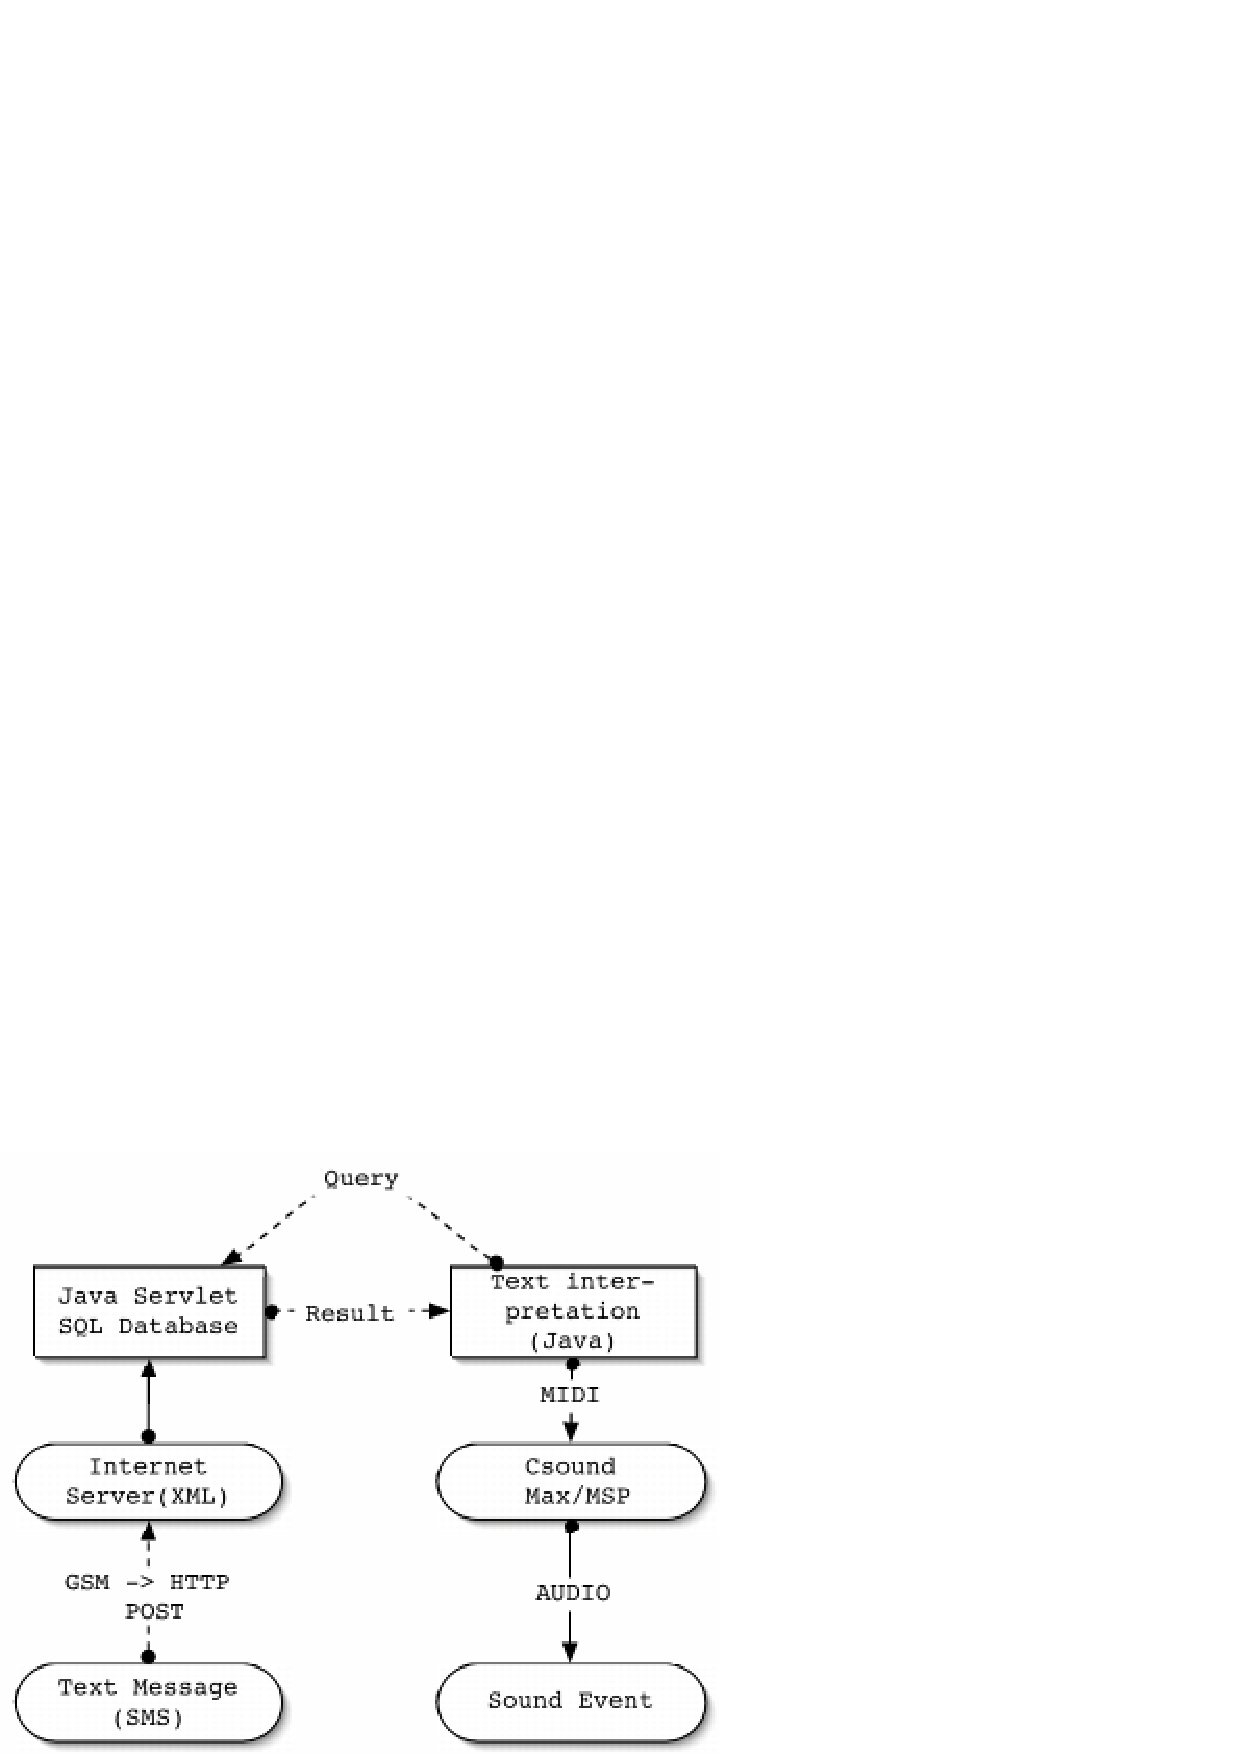
\includegraphics[width=0.45\textwidth]{img/ethsnd/Figure1}
\caption{Communication in the first version.} \label{model1}
\end{center}
\end{figure}

\subsection{Communication - first model}
\label{sec:comm-first}
In the first version, realised in August 2003,\footnote{See the audio   and video recording \emph{etherSound}/\emph{etherSound 2003}.} the communication between the participant and the system was accomplished according to Figure \ref{model1}. An SMS sent to a specified number was transformed to a XML file (eXtensible Markup Language, see \url{http://en.wikipedia.org/wiki/XML}) and transferred to a URL by a HTTP POST request. This part was handled through an external service. At the called URL, a JSP (Java Server Pages) was directing the POST data to a Java Bean \citep{j2ee} that handled the parsing of the data and the connection to a MySQL database in which it created a new entry with the relevant fields. 

It was due to security reasons at the museum where this version was realised that the HTTP request could not be handled locally. Instead, the local computer queried the server database for new entries on regular intervals.  After some testing, sending a SQL query once every second seemed like a reasonable time interval. Shorter time intervals didn't accomplish a perceivably quicker response time and, since the synthesis program was running on the same machine, I didn't want to use more processing and network activity than necessary for this task. After the text message had been processed, control signals where sent by \useGlosentry{glos:MIDI}{MIDI} to the synthesis engine. 

As is obvious from the recordings of the two versions, the sounds produced by the computer in this first version is very different from those in the second recording.

\begin{figure}[hbp]
  \begin{center}
    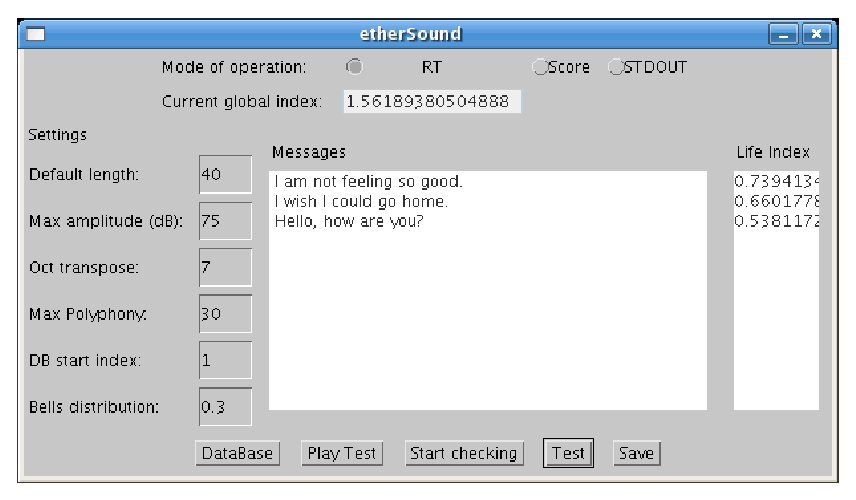
\includegraphics[width=0.9\textwidth]{img/ethsnd/MainGUI}
  \caption{Main GUI window for the \emph{etherSound} program.}
  \label{fig:main_gui}
\end{center}
\end{figure}

\subsection{Communication - current model}
Although the first version worked well and was fairly stable, it was a solution that required an external SMS processing service, and a local, reliable network connection. In order to make the piece more 'portable' and independent, the message receiving part was rebuilt. Using the gnokii API \citep{gnokii} it is relatively easy and reliable to connect a GSM phone to a computer and gain access to the storage and status of the phone which enables reception of the SMS messages locally. To still have the possibility to review the activities of transmission, the messages are, just as in the first model, written to a database. In other words, the client-server model is retained but on one and the same machine. Furthermore, the \useGlosentry{glos:MIDI}{MIDI} connection between the control application and the synthesis engine was replaced with Open Sound Control (OSC) \citep{osc, osc_web} for speed, reliability and flexibility, using the library JavaOSC (see \url{http://www.mat.ucsb.edu/~c.ramakr/illposed/javaosc.html}). 

\begin{figure}[hbp]
  \centering
  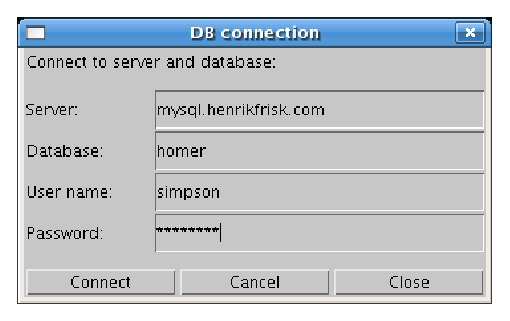
\includegraphics[width=0.5\textwidth]{img/ethsnd/DB_connection_window}
  \caption{Panel for connecting to the database.}
  \label{fig:DBpane}
\end{figure}

\subsection{The text analysis}
The program handling the text processing and the mapping of text to control signals for the sound synthesis is written in Java \citep{j2se} and features a simple but useful \index{GUI (Graphical User Interface)}Graphical User Interface (GUI) for control and feedback about the status of the system (see Figure \ref{fig:main_gui} and Figure \ref{fig:DBpane}).  

% It is in the mapping % between the text and the synthesis and sequencing of the sound events % that the musical potential of the system is constructed.  From the information extracted from the message control signals are generated which then influence (ordered from general to specific): 
\begin{itemize}
\item{The length of the whole event}
\item{The rhythm and articulation of the individual sound events}
\item{The pitch and character of individual sound events}
\end{itemize}
Controlling the timing of events there are two parameters; a local `life' index shaping the rhythms and the length of the current message and a global index that influences the current and subsequent `message-compositions'. The global index is a function of the current and previous messages local indexes. The local index is a result of a simple semantic analysis of the message. It indicates the message's relative structural complexity and allows the algorithm to discriminate between messages with a set of random letters and messages with real words and real sentences. The participant should be rewarded for the effort of writing a message with substance, where `substance' is defined here as a message with a credible average word length and a reasonable distribution of vowels within these words. In the analysis substitutions are made to allow for (i.e. not punish) idiomatic SMS writing such as `R u here?' or `C u 2 nite'. These examples are expanded into their `correct' equivalent. Standard abbreviations are also expanded. 

The local index is calculated by looking at the average length of words and the average number of syllables per word and comparing these with constants: 

\begin{equation}\label{index}
i_1=\frac{1}{(w(\frac{c}{w_c})-w_l)^{1/2}+1} \qquad i_2=\frac{1}{(w(\frac{s}{w_c})-s_l)^{1/2}+1}
\end{equation}

where $c$ and $s$ are the total number of characters and syllables, $w_c$ is the number of words in the current message, $w_l$ and $s_l$ are constants defining the `optimal' mean number of words/syllables. $w$ is a weight defined by 
\begin{equation}
w=\frac{1}{w_c-s_c+0.5}
\end{equation}

where $s_c$ is the total number of words that contains vowels. Through $w$, the index is decreased if the message contains words without vowels. The mean value of $i_1$ and $i_2$ is then multiplied by the arcus tangens of the number of words in relation to a third constant parameter, $o_w$, delimiting the optimal number of words per message\footnote{Since a SMS is limited to 160 characters these   constants are set according to what kind of message content should   be rewarded.} according to \eqref{life}.

\begin{equation} \label{life}
lifeIndex = \frac{i_1+i_2}{2}{\arctan (\frac{w_c}{o_w})}
\end{equation}

If we set $w_l$ to 4.5, $s_l$ to 2.0 and $o_w$ to 10 the result on four different messages can be seen from Table \ref{result}; the method distinguishes fairly well between nonsense and real words at a low computational cost. Similar or better results could conceivably be achieved in a number of different ways but this method appears to work well for the purpose.

  \begin{table}[!tbp]
    \begin{center}
      \begin{tabular}{l|r}
        \hline
        \textbf{Message} & \textbf{Life index} \\
        \hline
        \small{hello} & 0.18882 \\
        \hline
        \small{\textit{Hello, my name is Henrik}} & \textit{0.81032} \\
        \hline
        \small{hjdks la s duyfke jhsldf hasdfiw uehr jkdsl} & 0.14448 \\
        \hline
        \small{\textit{From fairest creatures we desire increase,}} & \textit{1.44618} \\
        \small{\textit{\ \ \ \ That thereby beautys rose might never}} & \\
        \hline
      \end{tabular}
      \caption{Life index for four different messages} \label{result}
    \end{center}
  \end{table}

  The total length of the music derived from the message is calculated   by multiplying a constant preset time with the local index. Any new   message received adds its local index to the instantaneous global   index which decreases exponentially at a set rate.\footnote{The rate     is context dependent. In a performance with improvisation it would     be shorter than in an installation.} If a message causes the   global index to reach maximum, it stops the playback of the current   message and begins playing back a precomposed pattern, sonically   different from the output of a typical message, for about 30 seconds   before resuming ordinary mode and starts playing back the message   that caused the break. This feature is added to reward collaborative   efforts. The global index controls mainly the density and the   overall volume of the output, but also the distribution of random   and stochastic processes in the synthesis. 

\subsection{The synthesis}

The synthesis engine is written as a Csound orchestra \citep{csound} (For more information on Csound see also \url{http://www.csounds.com/}). In the first versions of \emph{etherSound} Csound was running inside a Max/MSP (\url{http://www.cycling74.com/products/maxmsp.html}) patch through the use of the \texttt{csound$\sim$} object (see \url{http://www.csounds.com/matt/}). The Csound score for the message to be played back was sent to Max/MSP using OSC. Max/MSP was responsible for timing the note events and preparing valid information for the \texttt{csound$\sim$} object and the orchestra file associated with it. Due to processing power limitations only one message could be played back simultaneously; if a message was received before the previously received message had finished playing back, the new message would interrupt the current message (this can clearly be heard in the recording of the performance from 2003). In the latest version of the \emph{etherSound} software, instead of sending the Csound score events over OSC, they were sequenced and written to the standard output and sent to Csound through a UNIX pipe. Also, rather than limiting the number of voices by letting new messages crudely cut off currently playing messages the number of simultaneous voices available is now set in the \emph{etherSound} GUI (see Figure \ref{fig:main_gui}) and may be changed dynamically. The following discussion relates to the current version of \emph{etherSound}. 

\begin{figure}[!hbp]
  \centering
  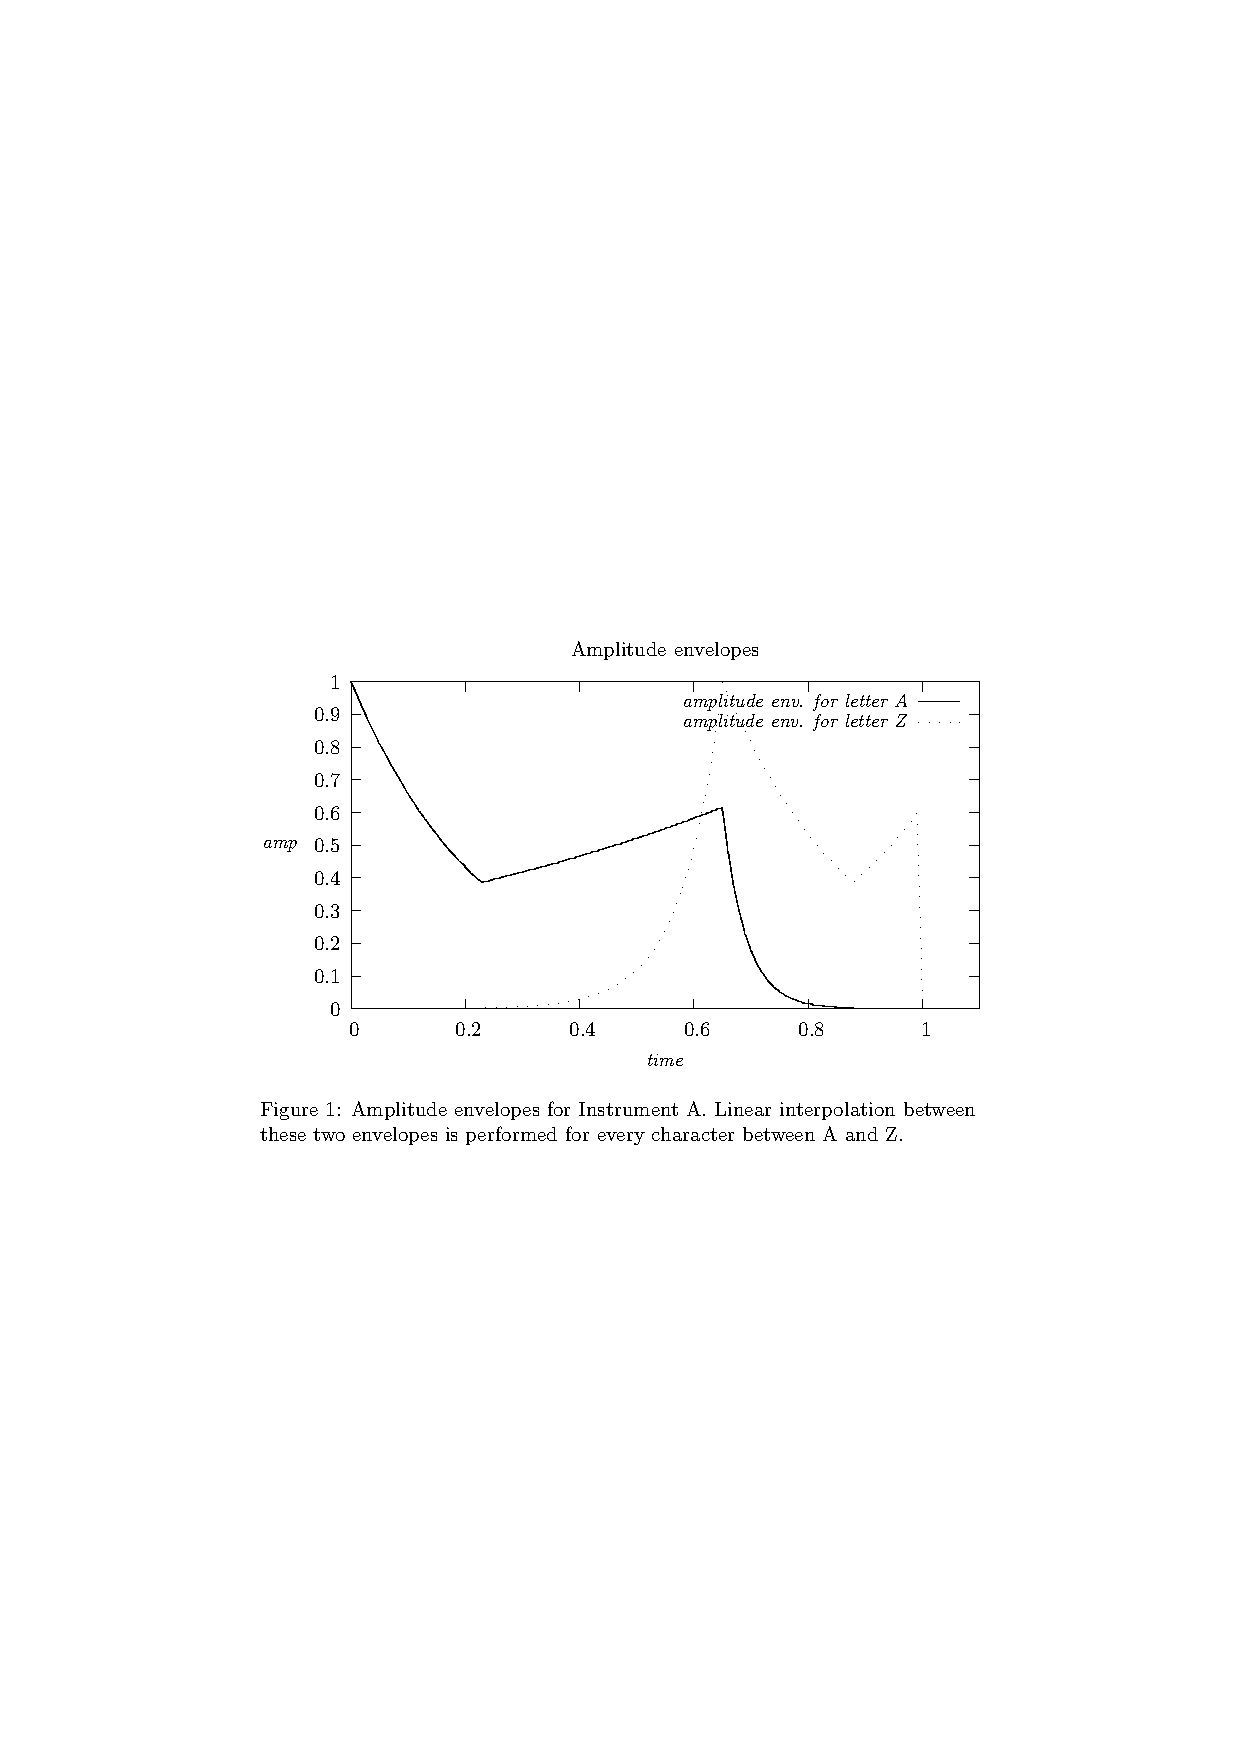
\includegraphics[trim=40mm 120mm 0mm 80mm, clip, height=50mm]{img/ethsnd/envelope}
  \caption{Amplitude envelopes for Instrument A. Linear interpolation
    between these two envelopes is performed for every character
    between A and Z.}
  \label{fig:envelope}
\end{figure}

All sounds heard in \emph{etherSound} are generated with FOF (Fonction d'Onde Formantique) synthesis as this technique is implemented in Csound \citep{fof,fof2}, using both samples and simple sine waves as sound sources. There are two distinct timbres played by two different instruments in each message-composition: (A) granulated samples of a male reading a text in English\footnote{An excerpt of the recording of   one of John Cage's lectures at Harvard College 1989.} and (B) a bell like sound whose formants are matched to and interpolated between the series of vowels in the text.  

\subsubsection{Instrument A} Every word of the message is considered one phrase or \emph{bar} of music in the resulting message composition. The number of beats per bar is approximately equal to the number of syllables in the word, where a syllable is defined as a vowel or group of consecutive vowels or a punctuation mark. The rhythmic subdivision of each bar is equal to the number of characters, including punctuation and white space, in each syllable. Thus, a one syllable word such as `my' followed by a white space results in a phrase consisting of one bar of one beat and two notes and one pause, i.e. three (eight-note) triplets of which the last is silent (see Table \ref{time}). If a word ends with a full stop, a comma, an exclamation mark or a question mark, more emphasis is put on the end of the bar containing the punctuation mark and the last note of the resulting phrase will be elongated. A note close to a vowel will more likely be accented than a note away from a vowel. 

The amplitude envelope curve of each note is related to the letter the note corresponds to. Envelopes are mapped linearly to characters; the letter `A' has a short attack and a long decay and the letter `Z' has a long attack and a short decay (see Figure \ref{fig:envelope}). The amount of overlapping between notes, i.e. the lengths of the notes, is influenced by the current life index \emph{and} the global index where higher values will result in longer notes and thus in smoother transitions between timbres. The notes of Instrument A do note have a perceivable pitch. Twenty-eight short sample buffers (typically 32.768 samples or approximately 0.7 seconds), one for each letter, are dynamically mapped one to one to the characters in each message. The FOF synthesis is used to granulate these samples, creating an erratic, non-tonal texture however still, in most cases, reminiscent of speech. 
\begin{figure}[!htb]
  \begin{center}
    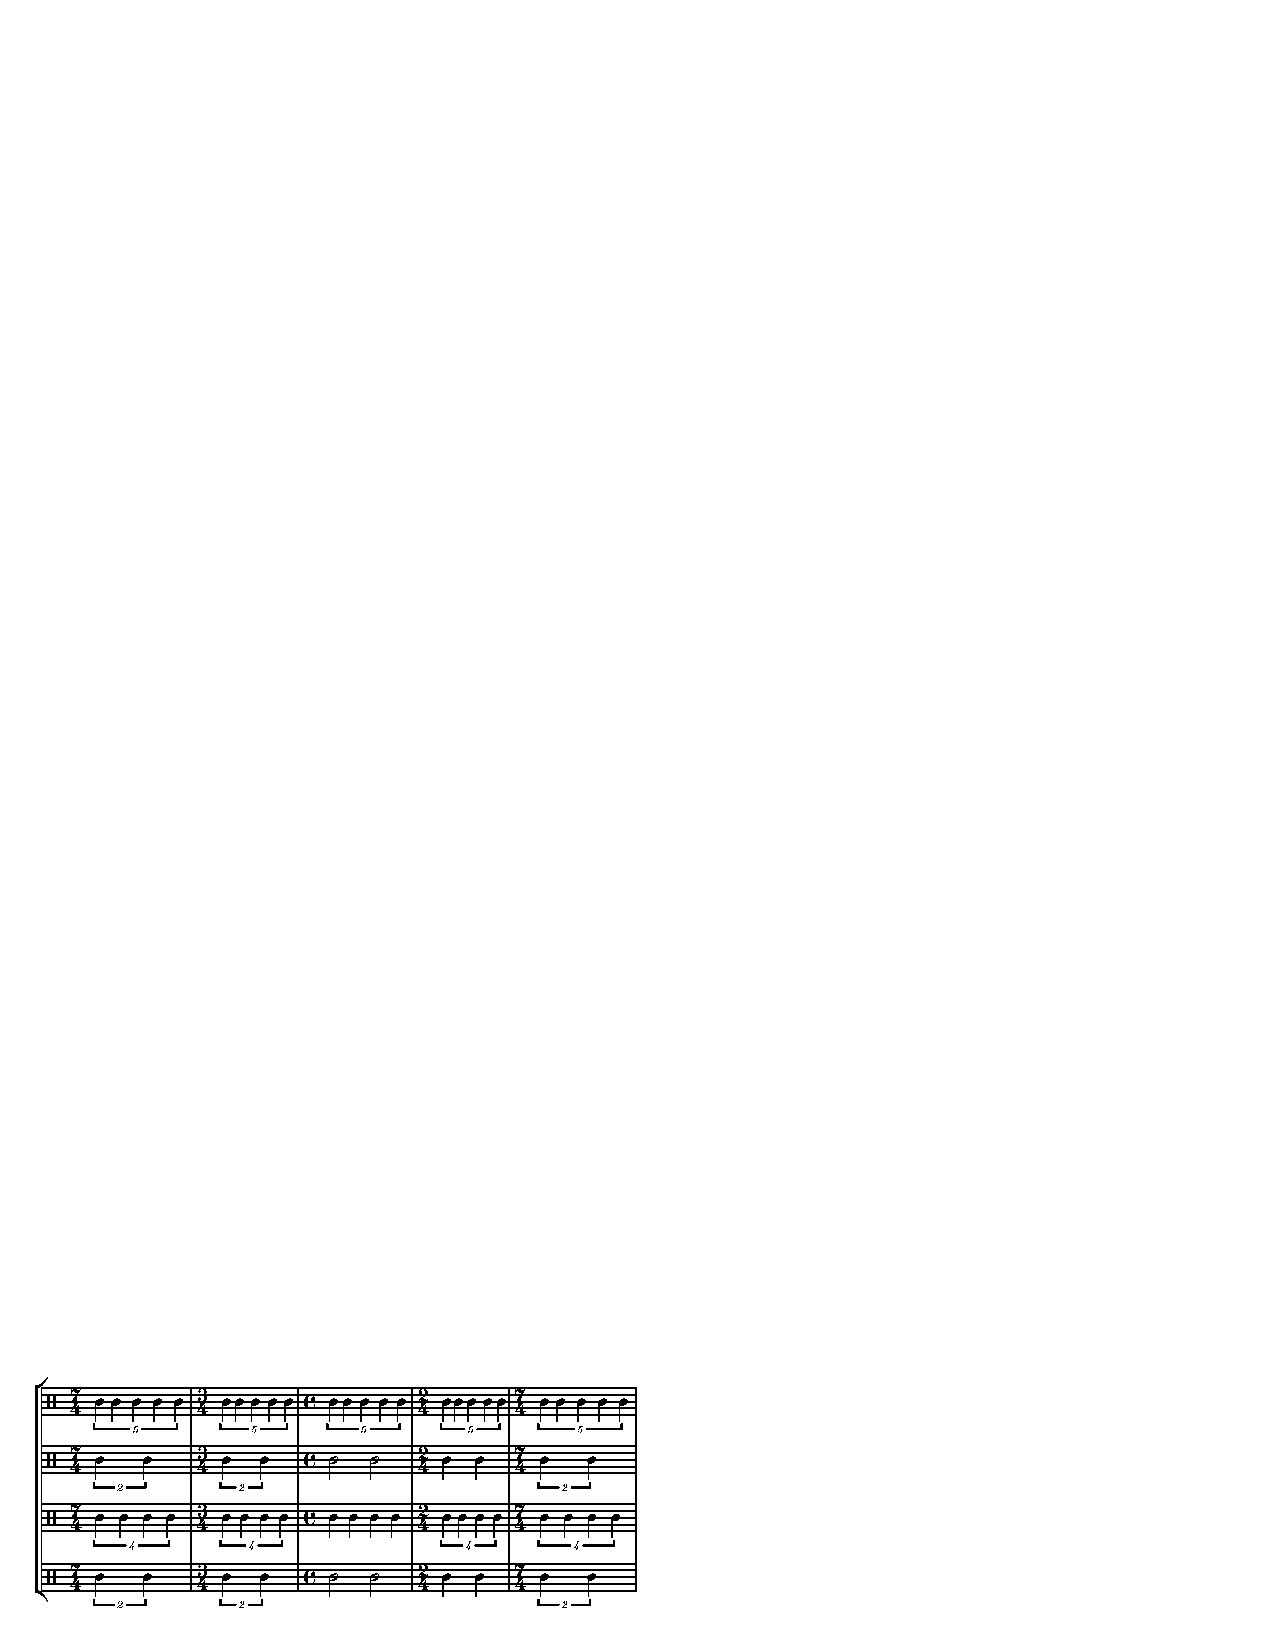
\includegraphics[width=0.8\textwidth]{img/ethsnd/harm}
    \caption{Rhythmic distribution of notes in Instrument B as a
      result of the message ``\emph{Hello, my name is
        Henrik.}''.} \label{time2}
  \end{center}
\end{figure}

\subsubsection{Instrument B}
The phrasing of the notes of the second instrument is somewhat more complex than that of Instrument A. This instrument has, at the most,\footnote{As already stated, the maximum number of voices is set based on what the   processing power of the system is.} as many voices as there are words in the message. An example of the rhythmic mapping of notes is shown in Figure \ref{time2}, the origin of which is the message in Table \ref{time}, with the polyphony limited to four voices. For this instrument the number of beats per bar (i.e. per word) is equal to the number of letters per word, including trailing punctuation marks and white space. If there are less words than the maximum polyphony, the number of voices is equal to the number of words; the first voice correspond to the first word, the second voice to the second word and so forth. For every bar, each voice has as many potential excitations as there are letters in the corresponding word. After the initial excitation, which will always be played, the likelihood that a given note will be played is related to the life index \emph{and} the global index: If the normalised sum of the local index and the global index is 0.5, half of the excitations will be performed. The amplitude envelope curve for the notes played by this instrument is either of a bell like character or of its inversion, and notes close to the beginning of a bar has a greater likelihood of being emphasised. 

\begin{figure}[!htb]
\begin{center}
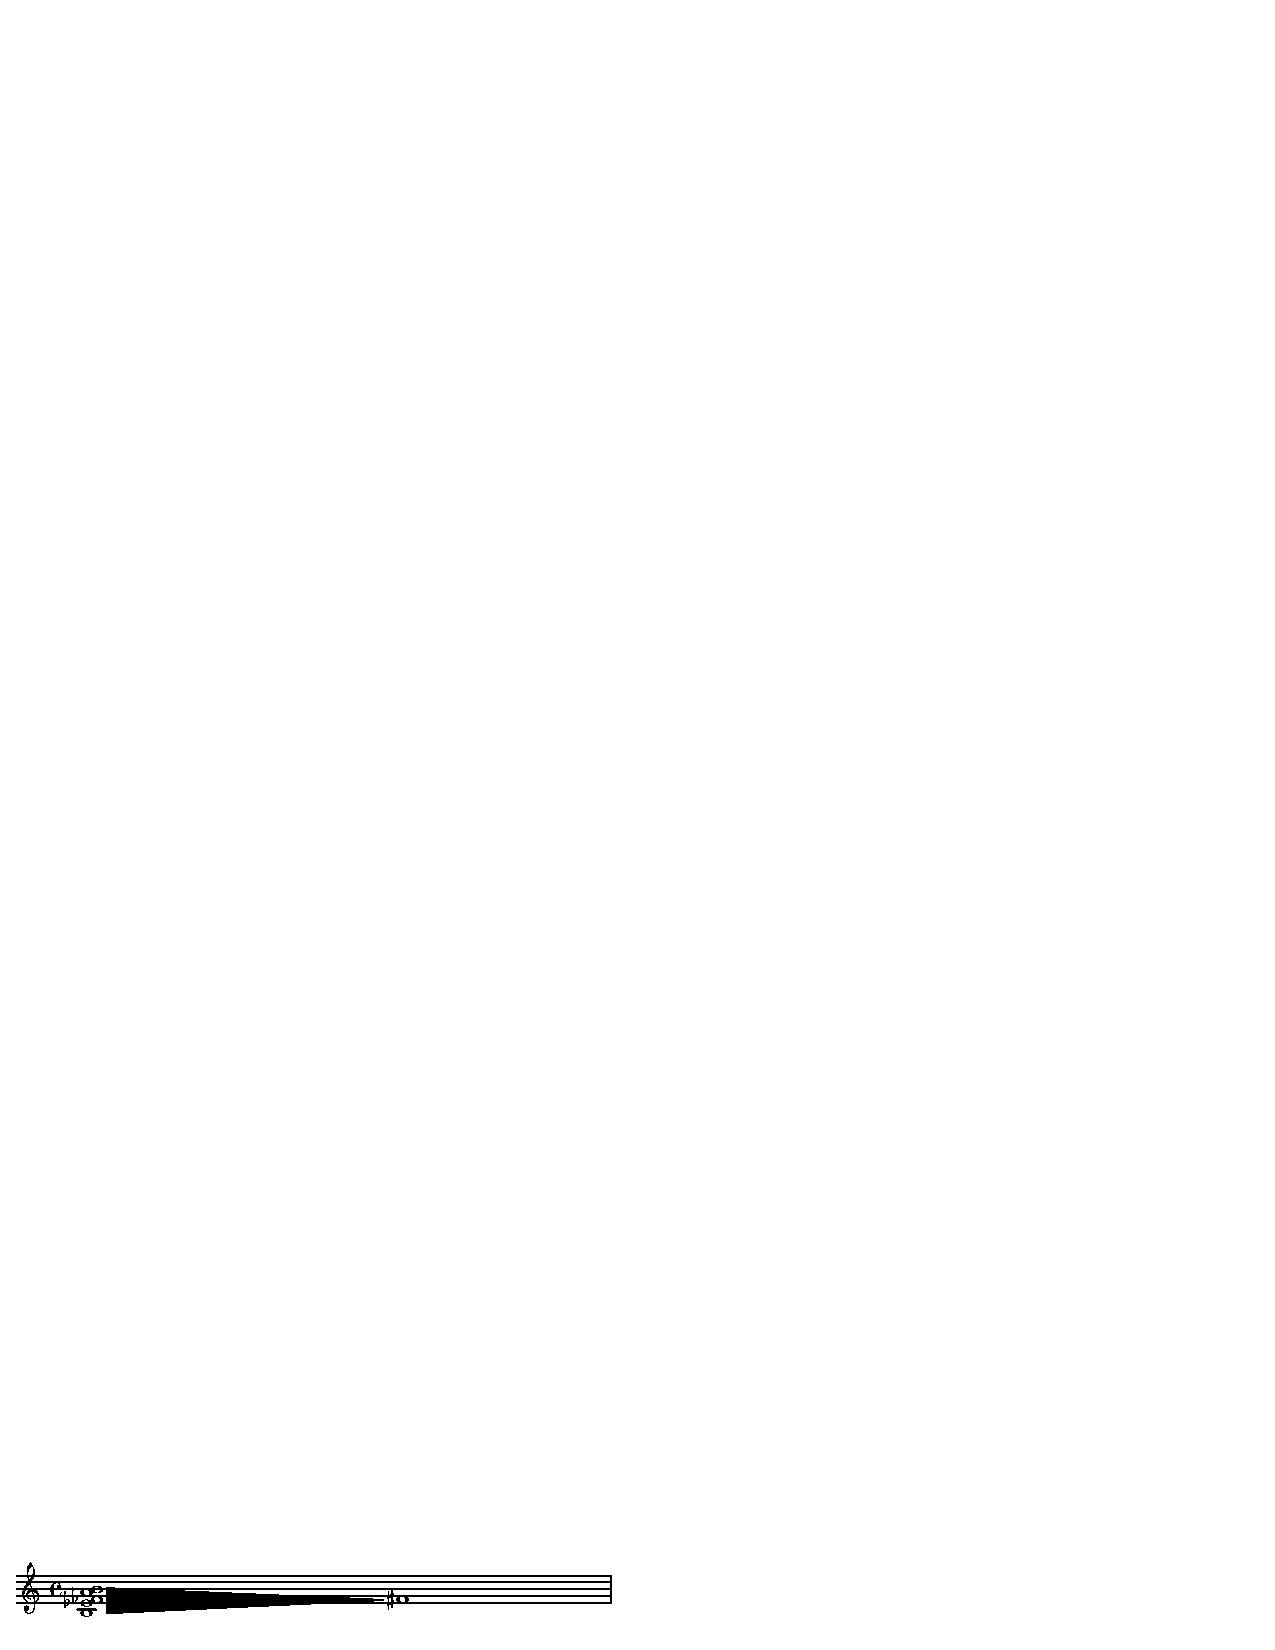
\includegraphics[width=0.8\textwidth]{img/ethsnd/chord}
\caption{Harmony for Instrument B as a result of the message
  ``\emph{Hello, my name is Henrik.}''.} \label{chord}
\end{center}
\end{figure}

The initial pitches are derived from the occurrence of certain key letters in the originating text.\footnote{For the sake of experiment   and variation, I am changing these 'key notes' for every performance   of \emph{etherSound}.} The first unique occurrence of one of the key letters, searched for from the first letter of the word corresponding to the current voice until the end of the message, becomes the initial pitch for each voice. If none is found the voice is deleted. The voicing of the initial chord is constructed so that the first voice will be the top note of the chord and consecutive voices will be laid out below this using octave transposition, aiming for the closest possible voicing. 
The exact micro-tonal center pitch between the highest and lowest note of the initial chord is then calculated (this would be the pitch `D' if the initial chord is a major third up from `C'). After the initial chord has been introduced, all voices begin a virtual glissando toward the center between the outer limits of the chord, creating micro-tonal variations, ending at a unison.\footnote{The same technique is used in   the composition \emph{Drive} (2003). The score for \emph{Drive}   shows the notation of the instantaneous (approximate) harmony at   five consecutive points in time ending at a B quarter of a tone   sharp.} For each excitation of each voice, the instantaneous value of the corresponding glissando sets the pitch for that excitation. The message from Table \ref{time} would result in the chord showed in Figure \ref{chord}---the initial chord and the glissandi towards the center pitch---if the max polyphony value is set to five or higher and the `key' characters were mapped by German note names (a to A, b to Bb, c to C, ... ,h to B and s to Eb). 
The timbre of the voices played by this instrument is shaped by the vowels contained in the message and the order in which they appear. For non real time processing this is achieved by synthesizing the first five formants of the first vowel found in the word corresponding to the current voice and then interpolating between the formant spectrum of the remaining vowels of the message (see Table \ref{vowel}). As this method is very expensive---it requires allocation of five times more voices---a cheaper alternative was used in the first real time versions of \emph{etherSound}. By modulating the formant center frequency of one single FOF voice using frequency modulation with the carrier and index signal frequencies derived from the vowel interpolation described above, the effect of molding the spectrum in a way related to the content of the message is retained. In the latest version the two methods are combined in order to achieve a greater sonic variation---all five formants are synthesised for every note and the formant center frequencies of some of the notes are also modulated. 
\subsection{Sound event generation and synthesis---conclusion} The two instruments offer two different interpretations of the message played back in parallel. As Instrument A performs a linear displacement within the message, Instrument B gives a snapshot image of the entire text at once, an image which is gradually dissolving over time. Metaphorically speaking, one instrument is modeling the discrete words and characters as they appear in time, the objective flow of the components of the message, and the other deals with the continuous meaning, or subjective understanding, of the message as it is interpreted in its entirety. Although the result can be rather complex and abstract it is my intention that certain conceptual elements of the input should be retained in the output. In the following section I will reflect on the issue of interaction within the context of \emph{etherSound} and to what extent my intentions of input-output correlation can be said to have been fulfilled. 
\section{Discussion and reflection} As has already been explained, the main issue for \emph{etherSound} is to allow for unconditioned participation. It comes natural that unconditioned perception should similarly be allowed for. More concerned with the collection of diverse input than I was in giving the contributor a sense of control or participation, in the first versions of \emph{etherSound} the message-compositions where much less dependent on input than what they are in the current version. My grounds for changing this and, in the current version letting the messages generate a musical event with a clear form stems from the wish to retain a perceptible connection - even though this connection may only be dismantled by the \emph{change} in output - between input and output. 
The process of designing the analysis and synthesis programs described above is to a considerable extent tantamount with the process of composing in the traditional meaning. In a sense, \emph{etherSound} is an algorithmic or ruled based composition\footnote{French composer   Michel Philippot and Italian composer Pietro Grossi were both   pioneers of algorithmic composition.} with stochastic elements, methods which have been explored by many composers for many years. In his book \textit{Formalized Music} composer Iannis \citet{xenakis71} offers a thorough investigation of the concept of stochastic music which came about as a reaction to the post serialistic music:

\begin{quote}
  For if, thanks to complexity, the strict, deterministic causality   which the neo-serialists postulated was lost, then it was necessary   to replace it by a more general causality, by a probabilistic logic   which would contain strict serial causality as a particular case   (p. 8). 
\end{quote}

But where in the case of Xenakis the results of the stochastic processes were strictly encoded into a score or a computer program, in \emph{etherSound} there is no score as such. The mapping between characters in the input, and synthesis and sequencing parameters used to produced the output is fixed in the program but no sound will be produced unless someone takes the action to provide the system with input. John Cage's non-deterministic music based on chance operations is another example in which events in some regard external to the composer is allowed a great influence on the final result. Cage's aesthetics were a means to remove \textit{intention} from the artistic expression. On the face of it there may be a conceptual resemblance between \emph{etherSound} and the non-determinism of Cage. However, in \emph{etherSound} it is precisely \textit{intention} that produces sound: The wish to participate is all that is needed. 

The choices that had to be made in the mapping of input to output in the program are the same kind of choices I make when I compose or improvise. I would call these compositional choices. They are made based on my musical experience and on what it is I want to achieve---for whatever reasons---at any one particular moment. The process of making these choices in the context of developing and designing interactive systems is well described by Camurri et al.: ``The designer of the performance introduces sound and music knowledge into the system, along with the compositional goals [..]'' \citep[Camurri, Richetti, and Trocca, 1999, as cited in][p. 373]{rowe01}. This fact, that compositional choices were made in the course of constructing \emph{etherSound}, does not necessarily make it into a `composition'. But before pondering more on the identity of \emph{etherSound}, what is the nature of its driving force, the interaction between the program, the \index{performer}performers and the participants? In what sense is \emph{etherSound} interactive? If the mapping is fixed in the program, what is the influence of the participant? 

\subsection{Interaction in \emph{etherSound}}
\label{sec:inter-emph}

\emph{etherSound} has been used in two different contexts. As a stand alone sound installation that users can interact with but also in combination with one or several improvising musicians playing acoustical instruments. The discussion that follows will primarily deal with the latter situation, which resembles a traditional concert but one in which the audience, apart from listening also may `play' the electronic instrument. As can be gathered from the description of the system given above, the sonic outcome of a received SMS is fairly strictly pre-conceived. On the individual level, only a limited amount of influence over detail is offered, and it is debatable whether \emph{etherSound} can be called an `instrument' at all. 
%%% Why would we like to call etherSound an instrument? %%%
This was however never the intention. It is the \emph{desire} to contribute to the whole that was intended to be the ruling factor, not the individuality of expression or the virtuosity of performance. But in that case, why not simply have a button that the users can press at will which generates a pseudo-random sequence of sonic events? Surely, this too would allow for unconditioned participation.
 
In the very first performance of \emph{etherSound}, on the day of the opening of the exhibition \emph{The Invisible Landscapes} in August 2003, due to a technical problem,\footnote{The problem was due to an   unknown inconsistency in how JSP (Java Server Pages), which I used   on the server to parse the messages, handled HTTP/POST requests when   the version of the HTTP differed between the caller and the   receiver.} as an emergency solution, I had implemented a version which basically worked like a button. I was unable to parse the actual contents of the SMS messages sent to the system (I merely obtained a notification that a message had been received). Rather than cancel the performance I had the program read an arbitrary number of words from a text file on my hard drive and use that as a `fake' message. Still, in the information about the installation and in the program notes for the concert, all of which had been prepared well in advance, it was stated that the system responded to the contents of the message when composing its output. After the concert a few of the listeners/participants came up to me and told me how clear they thought the connection between the SMS contents and the sounds were.  The expectancy of a correlation between input and output was so strong that, despite the fact that the actual mapping was completely random, the connection was created in the perception of the participant. This is not to say that `faking' interaction is practicable solution, but merely that expectation, hence information about (modes of) interaction, is an important factor. 

\emph{etherSound} is not interactive in the way that for example a computer game is interactive. Once the SMS has been sent, there is no way for the participant to alter or influence the sound. There is correlation between input and output in so far as short messages produce short message-compositions and vice versa. After having send a few messages, or after listening to a series of message-compositions, the participant will know what to expect and the ease-of-use is perhaps the greatest advantage of \emph{etherSound}. Interaction in the context of computers and technology is more or less synonymous with \textit{control}, or with the ability to change the prerequisites during the course of action. Or as put by George \citet{lewis00}: ``interactivity has gradually become a metonym for information retrieval rather than dialogue'' (p. 36). 
%%% What about 'dialogueâ' in etherSOund...  Is there real dialogue? %%%
Computer programs that are not interactive perform a task based on the information given to it at the outset. In interactive computer programs the parameters can be changed dynamically. By this definition and if we restrict the time frame to one message-composition, \emph{etherSound} is not really interactive or only interactive in a very limited sense. It does not allow the user to dynamically control the musical contour of the message-composition. It is more of a stochastic jukebox whose `play' button works by means of sending an SMS. 

But, if we expand our understanding of interaction and include readings that are more closely related to social interaction, which is not about control, but about exchange, about giving and taking, and about growing and establishing identity,\footnote{The role of social   interaction in human existence has a long philosophical history, in   recent years kept alive by Hannah Arendt and J\"{u}rgen Habermas.   This is discussed in more detail in the \emph{Music and Interaction}   section of this dissertation.} and we expand the time frame to include a series of message-compositions, we can come up with another analysis. If our general requirement for the definition of interaction is not limited to the subject's unbounded control over content (``information retrieval''), and the for this context specific requisite on interaction is not restrained to the participant-computer interaction, but also includes participant-participant and participant-performer interaction: Then \emph{etherSound} may well be said to manifest a form for dynamic interaction and the users that interact with it do indeed have influence.
%%% IS interaction the same as influence? %%%
In a recent performance (Copenhagen, August 2007) a participant sent a message that ended the concert.  Whether that was intended or not is less important than the actual consequence. The participant introduces a change in the musical context and, though he or she does not control the outcome of this change, the participant still in effect has the power of influence (influence rather than control) through interaction. 

What then are the consequences regarding interaction that may be drawn from working with \emph{etherSound} in the context of performance? If we begin by thinking about this piece as an improvised live performance: On an individual level the system \emph{etherSound} adds the ability for any member of the audience (who by virtue of being a part of the audience is already interacting with the performance) to interactively introduce a change to the sonic environment at any point, albeit with a very limited control over the outcome. Now, from my elevated perspective as a musician with a 15 years of professional experience I am in no position to tell what this situation means to someone who has never before participated in an improvised musical event. It may be incredibly dull or it may be the most exciting sensation. For me, as an improviser, the interaction as it is taking place here supplied that which the computer does not (and never will be able to?)  posses---the intention. The message-compositions are not dispersed randomly (as in a pseudo-random computer algorithm) but because someone wanted to participate. 
%%% To me this sounds a bit like our voting system. There is an intention on the part of the voter, there even might be some kind of influence. However, s/he has no idea at all what s/he will get after the elections %%%
When playing and I heard the sounds of a message-composition I felt honored that someone took the time to participate, like I was given a gift \footnote{the `gift' aspect is further discussed in \citealp{frisk05} and   \citealp{yoshida06}}.  Though these ideas, that the participation would supply me with a non-predictable, however not random, series of impulses, were part of the original conception of \emph{etherSound}, I had not anticipated the impact this situation would have on me. It is not easy to make general assumptions regarding interaction from this reflection. But, perhaps bordering on speculative, to me this shows the importance of moving beyond interaction as a deterministic mapping of stimulus to response. To let both parties involved in the interaction to create the object of interaction in order to intend it and embrace the improvisatory nature of interaction. %%% But is this determinism interaction? %%%

There is a number of different kinds of interaction going on in a performance of \emph{etherSound}, on many different levels. There is the low level interaction between the participant and the computer mediated through the mobile phone as well as higher levels of interaction between groups of participants and groups of \index{performer}performers. To summarise, in order to appreciate the nature of the interactive potential for \emph{etherSound} (i) time needs to be considered, (ii) expectation is an important factor and, (iii) information \emph{about} the processes taking place as a result of interaction (`meta-information' or the `grammar' of interaction) is absolutely essential. 

%%% More general remarks after reading thus far: Go deeper into the topic of interaction. E.g. (1) What about the difference between musician-composer, participant-composer, participant-musician? (2) Is intention a prerequisite for interaction and is therefore no real interaction possible with a computer? %%%

\subsection{The work identity of \emph{etherSound}}
\label{sec:ident-emph}

The question of the work identity is not merely a theoretical issue in this context of pure scholarly import. If the intention of \emph{etherSound} was to create an open-ended platform for public participation with a focus on interaction and, in the end, the result has more in common with a composition for instruments and computer, not only did the intention fail (which may be perfectly alright), but my personal objective, to use interaction as a way to open up the creative process and give up compositional control, failed. The latter may also be fine, but if in the long run there is a continuous discrepancy between artistic intentions and practical results this is likely to create personal and artistic frustration. 

Looking at the different agents involved in the production of musical content in \emph{etherSound}, the most obvious perspective to adopt (given that we talk about message-compositions) is that the participants are the composers and the computer along with the improvising musicians are the \index{performer}performers. This would make the SMS's the score(s). Musicologist Peter \citet[][]{kivy02} gives a definition of the musical score as ``a complex symbol system. From the performer's point of view it is a complex set of instructions for producing a performance of the musical work that it notates'' (p. 204). Applying this definition to \emph{etherSound}, we may extract (at least) two other plausible explanations to its structure:
%
\begin{enumerate} 
\item If the participants (SMS senders and improvising musicians) are   the \index{performer}performers, the instructions, the meta-information or the   `grammar' of the interaction constitute \emph{a} score. 
\item If the computer is the performer (which would turn the   participants into a kind of conductors) the computer program, i.e. the code,   in which the mapping between input and output is defined, would constitute   another \emph{version} of \emph{a} score. \end{enumerate}
%
According to the definition given, even if we regard the work from two or three different perspectives, there is a score. 
%%%The interesting point you’re coming at is that etherSound makes use of a singular score which seems like a kind of paradox %%%
If there in fact is a score of some sort in which the mapping is fixed and not subject to change through interaction, and further if the process of building this mapping scheme is similar or even equal to compositional processes, in what sense does \emph{etherSound} differ from a composition? First of all, and perhaps needless to say, Kivy's definition is by no means conclusive. Second, there is an important difference between a more traditional composition and a work such as \emph{etherSound} in the dimension of time, as the latter does not have a fixed beginning nor an end. Last, and most important, between the two contrasting musical work concepts `closed' or `pre-conceived', and `open' or `free' there is obviously a whole range of possibilities. And, as with so much other music and art, depending on \emph{when} and \emph{how} you look at the piece it will define itself at different points on the open-closed axis. It is part of the very nature of \emph{etherSound} that it flows and constantly redefines itself in the field ranging from the relative closeness form of the message-compositions and the openness of the large scale form of the improvisation. 

More than anything else \emph{etherSound} is an improvisation. The structure or the `language' for the improvisation may be different depending on your role, and the `score' (if it exists) is ``a recipe for possible music-making'' \citep[Evan Parker, as cited in][p. 81]{bailey92}. The compositional choices discussed above are a part, a for this piece necessary part, of the structure that makes possible the different entry points. Systematic and pre-conceived construction in one phase of a musical project does not have to limit the performative freedom or result in a closed `work'. On the contrary (and perhaps in opposition to the romanticised view on improvisation): Preparation for an improvised performance, even in free form jazz improvisation, is quite often highly structured and systematic. Improviser and jazz saxophonist Steve Lacy gives the following recollection of the early years of Cecil Taylor's career: ``And the results were as free as anything you could hear. But it was not done in a free way. It was built up very, very systematically [\ldots]'' \citep[Cited in][p.  81]{bailey92}.\footnote{It should be pointed out   that I make no comparison between \emph{etherSound} as music and the   music of Cecil Taylor.} Further, construction and pre-conception on the detailed level does not exclude that the whole is still open and self-generated: ``[E]ach of the numerous released recordings of, say, Coltrane's `Giant Steps,' regarded at the level of individual passages, is the result of careful preparation [\ldots]. At the same time, each improvisation, taken as a whole, maintains its character as unique and spontaneous'' \citep[p.  108]{lewis-1}. In both the recordings of \emph{etherSound} (2003 and 2007) the common `language' of the performing musicians is their background as jazz improvisers.
%%% So, the interaction goes in fact one way: it’s just a matter of seducing the performer (you) %%%
The language for the participants is the text and logic of SMS messages. And the intention to participate is what binds the two together. 

To conclude this discussion I would like to again turn to George \citeauthor{lewis-1} who, I believe, captures the essence of how form and structure is developed in improvised music: 
\begin{quotation}   My own view is that in analyzing improvisative musical activity or   behaviour in structural terms, questions relating to how, when, and   why are critical. On the other hand, the question of whether   structure exists in an improvisation---or for that matter, in any   human activity---often begs the question in a manner that risks   becoming not so much exegetic as pejorative. It should be axiomatic   that, both in our musical and in our human, everyday-life   improvisations, we interact with our environment, navigating through   time, place, and situation, both creating and discovering form. On   the face of it, this interactive, form-giving process appears to   take root and flower freely, in many kinds of music, both with and   without preexisting rules and regulations.  \citep[p. 117]{lewis-1} 
\end{quotation} 
From my personal horizon thinking about the work identity of \emph{etherSound}, I have gone full circle. At the outset I thought of it as nothing but a framework for improvisation in which I could allow myself to experiment with using the computer in a way distinctly different from how I was used to. Then, for many reasons of which one was the fact that it is precisely not \emph{axiomatic} that form may be created as well as constructed, I went into a phase of denial, in which I sought for a structure that would allow me to call \emph{etherSound} a `work'. Only to, in the end, arrive at the conclusion that, what it is, first and foremost, is an improvisation. 

%%%
%%% General remark: With whom is the audience actually interacting? (1) With the musicians on stage; (2) With etherSound; (3) With a computer; (4) With their cell phones; (5) With music (sounds)????? 
%%%

\section{End note}
\label{sec:endnote}

Whether or not the participants felt they had influence and whether this influence set creative energies in motion within the participant can only be proved, if at all, by performing empirical and statistical studies that are beyond my intentions and competence. What I can do however is reflect on my experiences of performing \emph{etherSound} at a number of occasions. And, based on my experiences as a performer---from that point of view---the participants were truly interacting with the music and they had genuine influence on the development of the performance. As an improviser in the context of a performance, I experience no difference between an initiative taken by one of the other musicians or one introduced by a participant---they are both of equal import. 
%%% Perhaps of equal import but at least the action-reaction among musicians continue and develop (deepen) %%%
Though I have programmed \emph{etherSound} myself, enough musically crucial aspects of the message-composition is unknown at the onset for any message-composition to hold potential for musical change. Obviously, the nature of the interface and the way the piece is programmed puts great limitations on the creative possibilities of the participants, especially were they to work with it repeatedly. That, however, does not mean that the individual, single act of participating does not harbor creative and interactive potential. Just as I, when improvising, cannot be certain how a musical initiative taken by me will influence the development of the music, the participant will not know either. 
%%% Is that really the same thing for you? %%%
Still---just to be absolutely clear about what it is we are talking about: Sending an SMS to \emph{etherSound} during a performance is obviously nothing like, not even closely related to, improvising on an instrument one has learned and mastered. In no way is this the point I am trying to make. The point I am making by this long detour of reflection is that, perhaps---and my own experience seems to corroborate this---a tiny atom of that which constitute the essence of the, at its best, flowering, form-giving process of improvisation, to use the words of George Lewis, can be shared by those whose participation is restricted to a mobile phone.
%%% Is this your main conclusion? %%%

However, and now we are approaching the weak spot of \emph{etherSound} as a platform for interaction, the more I play with and get to know my co-improvisers the easier it will be to predict the result of musical actions taken. For the participants there is currently only very limited possibilities for this kind of development to take place. Developing the expert performance aspect of a work whose objective is related to a notion of `equality of participation'---that all, regardless of prior (musical) training, should be allowed an equal chance to participate---is not un-problematic. If this goal is to be adhered to care must be taken to not accomplish the expert performance aspect at the expense of un-initiated participation. Adding a second layer of interaction would be one way to allow for the interested participant to acquire skills to more actively and consciously take part of a performance. This second layer could be implemented by making a phone call and interacting with the message-composition---changing the volume of it, the timbre, the tempo, etc.---in real-time, either by pressing digits on the phone or by voice control. 

In \emph{etherSound} in the performance context the audience is invited to take part of a group improvisation. Though the \emph{interaction-as-control} aspect of the participation is very limited the interactive action influences the music in a way similar to musical interaction in the context of improvisation. 
%%% I think I don’t agree (see previous remark) %%%
To summarise my own experiences with working with this project over a number of years, I can say that the sensation of improvising in a context where the audience can give sonic input---input that becomes an important part of the performance---is very rewarding. And this to an extent that I did not anticipate at the time the project started. A challenge for a future development of the concept, though the artistic implications of such development have to be carefully evaluated, would be to attempt at developing the participant control aspect of the interface without loosing the collaborative focus.

%%% So, what did etherSound teach you about the relation computer-music-interaction? What can you conclude in more general terms that will benefit not only your own artistic work but also others?  %%%

\newpage

\begin{landscape}
\centering
\begin{table}[!pt]
\begin{tabularx}{\linewidth}{|p{.8in}|X|X|X|X|X|X|X|X|X|X|X|X|X|X|X|X|X|X|X|X|X|X|X|X|X|}
\hline
&H & E & L & L & O &,& &M&Y& &N&A&M&E& &I&S& &H&E&N&R&I&K&.\\
\hline
\textit{bar}&\multicolumn{7}{|l|}{1} & \multicolumn{3}{|l|}{2} & \multicolumn{5}{|l|}{3} & \multicolumn{3}{|l|}{4} & \multicolumn{7}{|l|}{5}\\
\hline
\textit{beats per bar}&\multicolumn{7}{|c|}{3} & \multicolumn{3}{|c|}{1} & \multicolumn{5}{|c|}{2} & \multicolumn{3}{|c|}{1} & \multicolumn{7}{|c|}{3}\\
\hline
\textit{subdivision}&\multicolumn{2}{|c|}{2} & \multicolumn{3}{|c|}{3} & \multicolumn{2}{|c|}{2} & \multicolumn{3}{|c|}{3} & \multicolumn{2}{|c|}{2} & \multicolumn{3}{|c|}{3} & \multicolumn{3}{|c|}{3} & \multicolumn{2}{|c|}{2} & \multicolumn{3}{|c|}{3} & \multicolumn{2}{|c|}{2}\\
\hline
\textit{accents}& & \textgreater & & &\textgreater & & & & \textgreater& & & \textgreater& &\textgreater & &\textgreater& & & & \textgreater& & &\textgreater&\textgreater& \\
\hline
\end{tabularx}
\caption{Rhythmic distribution of notes in Instrument A.Influence of vowels on four consecutive voices of Instrument B.} \label{time}
\end{table}

\centering
\begin{table}[!pt]
\begin{tabularx}{\linewidth}{|p{.8in}|X|X|X|X|X|X|X|X|X|X|X|X|X|X|X|X|X|X|X|X|X|X|X|X|X|}
\hline
&H & E & L & L & O &,& &M&Y& &N&A&M&E& &I&S& &H&E&N&R&I&K&.\\
\hline
\textit{voice 1}&\multicolumn{3}{|c|}{E} & \multicolumn{3}{|c|}{O} & \multicolumn{3}{|c|}{Y} & \multicolumn{3}{|c|}{A} & \multicolumn{3}{|c|}{E} & \multicolumn{3}{|c|}{I} & \multicolumn{3}{|c|}{E} & \multicolumn{4}{|c|}{I}\\
\hline
\textit{voice 2}& \multicolumn{4}{|c|}{Y} & \multicolumn{4}{|c|}{A} & \multicolumn{4}{|c|}{E} & \multicolumn{4}{|c|}{I} & \multicolumn{4}{|c|}{E} & \multicolumn{5}{|c|}{I}\\
\hline
\textit{voice 3}& \multicolumn{5}{|c|}{A} & \multicolumn{5}{|c|}{E} & \multicolumn{5}{|c|}{I} & \multicolumn{5}{|c|}{E} & \multicolumn{5}{|c|}{I}\\
\hline
\textit{voice 4}& \multicolumn{8}{|c|}{I} & \multicolumn{8}{|c|}{E} & \multicolumn{9}{|c|}{I}\\
\hline
\end{tabularx}
\caption{Influence of vowels on four consecutive voices of Instrument B.} \label{vowel}
\end{table}

\end{landscape}

%%% Local Variables: 
%%% mode: latex
%%% TeX-master: "../ImprovisationComputersInteraction"
%%% End: 
